% This is a simple sample document.  For more complicated documents take a look in the exercise tab. Note that everything that comes after a % symbol is treated as comment and ignored when the code is compiled.

\documentclass{article} % \documentclass{} is the first command in any LaTeX code.  It is used to define what kind of document you are creating such as an article or a book, and begins the document preamble

\usepackage{amsmath} % \usepackage is a command that allows you to add functionality to your LaTeX code
\usepackage{tikz}
\usetikzlibrary{calc,matrix}

\title{Simple Sample} % Sets article title
\author{My Name} % Sets authors name
\date{\today} % Sets date for date compiled

% The preamble ends with the command \begin{document}
\begin{document} % All begin commands must be paired with an end command somewhere
\maketitle % creates title using information in preamble (title, author, date)

\begin{align*}
&Cartesian                      &               &Spherical\\
x(r, \varphi, \theta)&=           &r(x,y,z)&=\\
y(r, \varphi, \theta)&=           &\varphi(x,y,z)&=\\
z(r, \varphi, \theta)&=           &\theta(x,y,z)&=\\
\\
\text{basis}\\
\end{align*}
$$\mathbf{r} = x\hat{x} + y\hat{y} +z\hat{z}  
= x(r, \varphi, \theta)\ \hat{x} +y(r, \varphi, \theta)\ \hat{y} +z(r, \varphi, \theta)\ \hat{z}\\$$
\begin{align*}
\frac{\partial \vec{r}}{\partial x}&=\vec{x}=     &\frac{\partial \vec{r}}{\partial r}&=\vec{r}=\\
\frac{\partial \vec{r}}{\partial y}&=\vec{y}=     &\frac{\partial \vec{r}}{\partial \varphi}&=\vec{\varphi}=\\
\frac{\partial \vec{r}}{\partial z}&=\vec{z}=     &\frac{\partial \vec{r}}{\partial \theta}&=\vec{\theta}=\\
\end{align*}
$$\mathbf{r} = r(x,y,z)\ \vec{r} + \varphi(x,y,z)\ \vec{\varphi} + \theta(x,y,z)\ \vec{\theta}
=r\vec{r} + \varphi \vec{\varphi} + \theta \vec{\theta}$$
\begin{align*}
\frac{\partial \vec{r}}{\partial x}&=\vec{x}=     &\frac{\partial \vec{r}}{\partial r}&=\vec{r}=\\
\frac{\partial \vec{r}}{\partial y}&=\vec{y}=     &\frac{\partial \vec{r}}{\partial \varphi}&=\vec{\varphi}=\\
\frac{\partial \vec{r}}{\partial z}&=\vec{z}=     &\frac{\partial \vec{r}}{\partial \theta}&=\vec{\theta}=\\
\end{align*}

Notice:
$$\frac{\partial \mathbf{r}}{\partial r} = \vec{r} = \partial_r x \ \hat{x} + \partial_r y \ \hat{y} + \partial_r z \ \hat{z}$$

\[
J_{xyz \rightarrow r \varphi \theta} =
\frac{\partial(x,y,z)}{\partial(r, \varphi, \theta)} =\\
\begin{bmatrix}
\partial_r x & \partial_{\varphi} x & \partial_{\theta} x\\
\partial_r y & \partial_{\varphi} y & \partial_{\theta} y\\
\partial_r z & \partial_{\varphi} z & \partial_{\theta} z\\
\end{bmatrix}
\]


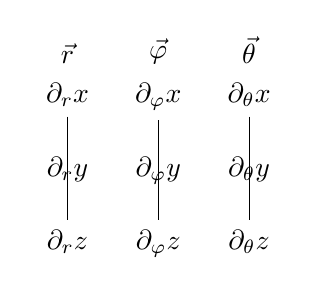
\begin{tikzpicture}[>=stealth]
  \matrix [%
    matrix of math nodes,
    column sep=1em,
    row sep=1em
  ] (Jacobian) {%
  \partial_r x & \partial_{\varphi} x & \partial_{\theta} x\\
  \partial_r y & \partial_{\varphi} y & \partial_{\theta} y\\
  \partial_r z & \partial_{\varphi} z & \partial_{\theta} z\\
  };

  \path (Jacobian-1-1) edge (Jacobian-3-1)
        (Jacobian-1-2) edge (Jacobian-3-2)
        (Jacobian-1-3) edge (Jacobian-3-3);
  {\node[anchor=south] at (Jacobian-1-1.north) {$\vec{r}$};};
  {\node[anchor=south] at (Jacobian-1-2.north) {$\vec{\varphi}$};};
  {\node[anchor=south] at (Jacobian-1-3.north) {$\vec{\theta}$};};
\end{tikzpicture}


\end{document} % This is the end of the document